%!tex root = ../main.tex
%% Background
%%
\section{Background}
To understand the chapter \ref{}, in this section we introduce relevant terminology and concepts.

In the first section (\ref{sec:distributed_computing}) of this chapter, we discuss about the essential concepts in the theory of distributed computing.
The section aims to explain the meaning of distributed computing and gives an introduction to the main model of distributed computing, \emph{message passing model}, from which many of the researched models inherit from.

The second and third sections discuss about the Port number model and local model respectively.
These are widely used models in the field and they are strongly related to the research showed in this paper.

We are trying to find lower bound proofs for LCL-problems in this paper, therefore it is essential to include a section entirely for them.
The fourth section (\ref{sec:lcl_problems}) is dedicated to LCL-problems.

Finally, in the last section (\ref{sec:previous_research}), we talk about previous research in the field and research that are more related to this thesis.

\subsection{Distributed computing} \label{sec:distributed_computing}
Computing or processing a computer program in several identical or different computation nodes is called distributed computing.
It is similiar to running a computer program that contains multiple concurrent tasks, but in distributed computing there are higher level tasks that are distributed to different computer nodes.

Computation nodes are connected to each others with communication channels.
These communication channels carry data from node to another node.
Together, nodes and communication channels form a network.
The best way to visualize these networks is by drawing a graph in which the nodes represent computing nodes and edges represent the communication channels.

\begin{figure}[h]
  \centering
  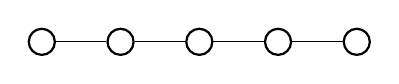
\begin{tikzpicture}[every node/.style={circle,thick,draw}]
  \node (1) {};
  \node (2) [ right of=1] {};
  \node (3) [ right of=2] {};
  \node (4) [ right of=3] {};
  \node (5) [ right of=4] {};
  \draw (1) -- (2);
  \draw (2) -- (3);
  \draw (3) -- (4);
  \draw (4) -- (5);
\end{tikzpicture}
\caption{Example of a distributed network.}
\label{fig:graph1}
\end{figure}

According to Lamport \cite{DBLP:books/el/leeuwen90/LamportL90}, in the area of distributed computing, the term \emph{model} denotes a view or abstract representation of a distributed system.
There are multiple different computation models used in distributed computing.
The most important main category of distributed computation models is \emph{process models}.
In process models, the work or activities are represented as concurrently executed processes that execute their instructions sequentially.
The main way to distinguish different process models from each other is to categorise them by the method they use to communicate with each other (\emph{interprocess communication}).
\cite{DBLP:books/el/leeuwen90/LamportL90}

Message passing models are a form of process model.
They are widely researched, for example ... \todo{add references to papers that research or use message passing models}
In the model, processes communicate by adding a message to message queue, wheter it is a shared or a process specific, and the recipient process removes the message (dequeues) from the message queue.
\cite{DBLP:books/el/leeuwen90/LamportL90}


%The following two sections (\ref{sec:port_number_model} and \ref{sec:local_model} ) talk about different forms of message passing models that are highly relative to this paper.

%In the theory of distributed computing, it is common to use terminology and concepts from graph theory as networks are basically graphs.
%With formal definitions, we can discuss more about the structure of distributed networks and reason features of those networks.
%We can further construct proofs of different theorems and so on. \todo{Fix this paragraph}

The algorithms that are executed in distributed fashion, are called distributed algorithms. \todo{where to write about distributed algorithms?}
%A distributed algorithm is a specific type of algorithm that is executed in distributed fashion.
Specifically, each node executes the same algorithm.

\todo{write about computation models, why they exist}

%\subsection{Message passing model}
\subsection{Port Number model} \label{sec:port_number_model}
\subsection{LOCAL model} \label{sec:local_model}
\subsection{LCL problems} \label{sec:lcl_problems}
\subsection{Previous research} \label{sec:previous_research}
\todo{Especially LCL classification research}
\clearpage
